\documentclass[11pt]{article} 
\usepackage[english]{babel}
\usepackage[utf8]{inputenc}
\usepackage[margin=0.5in,top=0.5in,bottom=0.75in]{geometry}
\usepackage{amsmath}
\usepackage{amsthm}
\usepackage{amsfonts}
\usepackage{amssymb}
\usepackage[usenames,dvipsnames]{xcolor}
\usepackage{graphicx}
\usepackage[siunitx]{circuitikz}
\usepackage{tikz}
\usepackage[colorinlistoftodos, color=orange!50]{todonotes}
\usepackage{hyperref}
\usepackage[numbers, square]{natbib}
\usepackage{fancybox}
\usepackage{epsfig}
\usepackage{soul}
\usepackage[framemethod=tikz]{mdframed}
\usetikzlibrary{positioning, automata, backgrounds}
\usepackage{tikz}\usetikzlibrary{arrows.meta,backgrounds,calc,quotes}
\usepackage[shortlabels]{enumitem}
\usepackage[version=4]{mhchem}
\usepackage{multicol}
\usepackage{forest}
\usepackage{mathtools}
\usepackage{comment}
\usepackage{enumitem}
\usepackage[utf8]{inputenc}
\usepackage[linesnumbered,ruled,vlined]{algorithm2e}
\usepackage{listings}
\usepackage{color}
\usepackage[numbers]{natbib}
\usepackage{subfiles}
\usepackage{tkz-berge}


\newtheorem{prop}{Proposition}[section]
\newtheorem{thm}{Theorem}[section]
\newtheorem{lemma}{Lemma}[section]
\newtheorem{cor}{Corollary}[prop]

\theoremstyle{definition}
\newtheorem{definition}{Definition}

\theoremstyle{definition}
\newtheorem{required}{Problem}
\newtheorem*{requiredHC}{Problem HC}

\theoremstyle{definition}
\newtheorem{ex}{Example}

\newcommand{\interval}[4]{\draw (#2, #1) -- (#3, #1); % Usage: \interval{height}{start}{end}{label}
\draw (#2, #1-0.11) -- (#2, #1+0.11); % draw left whisker
\draw (#3, #1-0.11) -- (#3, #1+0.11); % draw right whisker
\node[] at (#2-0.25, #1) {#4};
}

\tikzset{>={Stealth[length=7pt]}}
\tikzset{
    vertex/.style={circle,draw,minimum size=16,inner sep=0pt,font=\normalsize},
    edgelabel/.style={rectangle,draw=none,font=\footnotesize,outer sep=0pt},
    every node/.style={vertex},
    every edge quotes/.append style={edgelabel},
    every to/.append style={every node/.style={edgelabel}},
    wide/.style={line width=4pt,>={Stealth[length=18pt]}},
    directed/.style={arrows={->},font=\small},
    caption/.style={text width=6cm,align=center,rectangle,draw},
}


\setlength{\marginparwidth}{3.4cm}
%#########################################################

%To use symbols for footnotes
\renewcommand*{\thefootnote}{\fnsymbol{footnote}}
%To change footnotes back to numbers uncomment the following line
%\renewcommand*{\thefootnote}{\arabic{footnote}}

% Enable this command to adjust line spacing for inline math equations.
% \everymath{\displaystyle}

% _______ _____ _______ _      ______ 
%|__   __|_   _|__   __| |    |  ____|
%   | |    | |    | |  | |    | |__   
%   | |    | |    | |  | |    |  __|  
%   | |   _| |_   | |  | |____| |____ 
%   |_|  |_____|  |_|  |______|______|
%%%%%%%%%%%%%%%%%%%%%%%%%%%%%%%%%%%%%%%

\title{
\normalfont \normalsize 
\textsc{CSCI 3104 Fall 2022 \\ 
Instructors: Prof. Grochow and Nagesh} \\
[10pt] 
\rule{\linewidth}{0.5pt} \\[6pt] 
\huge Problem Set 2 \\
\rule{\linewidth}{2pt}  \\[10pt]
}
%\author{}
\date{}

\begin{document}

\definecolor{processblue}{cmyk}{0.96,0,0,0}
\definecolor{processred}{rgb}{200, 0, 0}
\definecolor{processgreen}{rgb}{0, 255, 0}
\DeclareGraphicsExtensions{.png}
\DeclareGraphicsExtensions{.gif}
\DeclareGraphicsExtensions{.jpg}

\maketitle


%%%%%%%%%%%%%%%%%%%%%%%%%
%%%%%%%%%%%%%%%%%%%%%%%%%%
%%%%%%%%%%FILL IN YOUR NAME%%%%%%%
%%%%%%%%%%AND STUDENT ID%%%%%%%%
%%%%%%%%%%%%%%%%%%%%%%%%%%
\noindent
Due Date \dotfill September 12, 2022 8pm MT\\
Name \dotfill \textbf{Tyler Huynh} \\
Student ID \dotfill \textbf{109603994} \\
Collaborators \dotfill \textbf{List Your Collaborators Here}

\tableofcontents

\section*{Instructions}
\addcontentsline{toc}{section}{Instructions}

 \begin{itemize}
	\item The solutions \textbf{should be typed}, using proper mathematical notation. We cannot accept hand-written solutions. \href{http://ece.uprm.edu/~caceros/latex/introduction.pdf}{Here's a short intro to \LaTeX.}
	\item You should submit your work through the \textbf{class Canvas page} only. Please submit one PDF file, compiled using this \LaTeX \ template.
	\item You may not need a full page for your solutions; pagebreaks are there to help Gradescope automatically find where each problem is. Even if you do not attempt every problem, please submit this document with no fewer pages than the blank template (or Gradescope has issues with it).

	\item You are welcome and encouraged to collaborate with your classmates, as well as consult outside resources. You must \textbf{cite your sources in this document.} \textbf{Copying from any source is an Honor Code violation. Furthermore, all submissions must be in your own words and reflect your understanding of the material.} If there is any confusion about this policy, it is your responsibility to clarify before the due date. 

	\item Posting to \textbf{any} service including, but not limited to Chegg, Reddit, StackExchange, etc., for help on an assignment is a violation of the Honor Code.

	\item You \textbf{must} virtually sign the Honor Code (see Section \ref{HonorCode}). Failure to do so will result in your assignment not being graded.
\end{itemize}


\section*{Honor Code (Make Sure to Virtually Sign)} \label{HonorCode}
\addcontentsline{toc}{section}{Honor Code (Make Sure to Virtually Sign)}
\hypertarget{HonorCode}{}

\begin{requiredHC}
\begin{itemize}
\item My submission is in my own words and reflects my understanding of the material.
\item Any collaborations and external sources have been clearly cited in this document.
\item I have not posted to external services including, but not limited to Chegg, Reddit, StackExchange, etc.
\item I have neither copied nor provided others solutions they can copy.
\end{itemize}

%\noindent In the specified region below, clearly indicate that you have upheld the Honor Code. Then type your name. 
\end{requiredHC}

\begin{proof}[Agreed (signature here).]
%% Typing "I agree to the above," followed by your name is sufficient.
\end{proof}


\newpage
\setcounter{section}{2}
\section{Standard 3 -- Dijkstra's Algorithm}

\subsection{Problem~\ref{dij}}
\begin{required}\label{dij}

Consider the undirected weighted graph $G(V, E, w)$ pictured below. Work through Dijkstra's algorithm on the following graph, using the source vertex $a$. 
\textbf{Note: }In order to get full credits consider the following:
\begin{itemize}
    \item Clearly include the contents of the priority queue, the distance from $a$ and the parent of each vertex at each iteration.
    \item If you use a table to store the distances, clearly label the keys according to the vertex names rather than numeric indices (i.e., \texttt{dist[`B']} is more descriptive than \texttt{dist[`1']}).
    \item You do \textbf{not} need to draw the graph at each iteration, though you are welcome to do so. [This may be helpful scratch work, which you do not need to include.]
    \item Finally represent the shortest path graph.
\end{itemize}

\begin{center}
	\begin{tikzpicture}[scale=4]
        \node (a) at (-0.5,0) {$a$};
        \node (b) at ($ (0,0) + ( 60:1)$) {$b$};
		\node (f) at ($ (0,0) + (-30:0)$) {$f$};
		\node (g) at ($ (0,0) + ( -120:0.5)$) {$g$};
        \node (d) at ($ (g) + ( 2,0)$) {$d$};
		\node (c) at ($ (f) + ( 1,0)$) {$c$};
		\node (e) at ($ (c) + ( 1,0)$) {$e$};
        
		\draw (a) to["5"] (b);
        \draw (a) to["12"] (g);
        \draw (b) to["3"] (e);
        \draw (b) to["5"] (c);
		\draw (b) to["7"] (f);
        \draw (c) to["8"] (f);
        \draw (c) to["1"] (e);
        \draw (e) to["10"] (d);
        \draw (d) to["3"] (g);
\end{tikzpicture}
\end{center}

\begin{proof}[Answer]
Using Dijkstra's algorithm on this graph, starting from vertex "a", we will implement a priority queue as per what Dijkstra's algorithm does. \\

\textbf{The algorithm itself:}\\
We will first initialize a priority queue where the weights of each vertex will be set to infinity as there are no weights associated with it: \\
\begin{center}
\begin{tabular}{ | c | c | c | c | c | c | c | c | }
 \hline
 Parent:& null & null & null & null & null & null & null\\ 
 \hline
 Distances:& a & b & c & d & e & f & g\\  
 \hline
 Weights: & $\infty$ & $\infty$ & $\infty$ & $\infty$ & $\infty$ & $\infty$ &$\infty$\\
  \hline
\end{tabular}
\end{center}
\begin{center}
Priority Queue: []
\end{center}

We will now push the vertex of "a" as it is our starting vertex to our priority queue:  \\
\begin{center}
\begin{tabular}{ | c | c | c | c | c | c | c | c | }
 \hline
 Parent:& null & null & null & null & null & null & null\\ 
 \hline
 Distances:& a & b & c & d & e & f & g\\  
 \hline
 Weights: & $\infty$ & $\infty$ & $\infty$ & $\infty$ & $\infty$ & $\infty$ &$\infty$\\
  \hline
\end{tabular}
\end{center}
\begin{center}
Priority Queue: [(a, 0)]
\end{center}

From the vertex of "a" we can see the vertices of both "b" and "g" with distances of 5 and 12 respectively. We will pop off the vertex of "a" and push onto the vertices of "b" and "g" and update the parents vertexes.  \\
\begin{center}
\begin{tabular}{ | c | c | c | c | c | c | c | c | }
 \hline
 Parent:& null & a & null & null & null & null & a\\ 
 \hline
 Distances:& a & b & c & d & e & f & g\\  
 \hline
 Weights: & $0$ & $\infty$ & $\infty$ & $\infty$ & $\infty$ & $\infty$ &$\infty$\\
  \hline
\end{tabular}
\end{center}
\begin{center}
Priority Queue: [(b, 5 ), (g, 12)]
\end{center}

From the vertex of "b" we can see the vertices of "c", "f", and "e". We will pop off the vertex of "b" and push onto our priority queue the vertices of "c", "f", and "e". The distances of the vertexes will be updated from that starting vertex of "a".\\
\begin{center}
\begin{tabular}{ | c | c | c | c | c | c | c | c | }
 \hline
 Parent:& null & a &  b & null & b & b & a\\ 
 \hline
 Distances:& a & b & c & d & e & f & g\\  
 \hline
 Weights: & $0$ & $5$ & $\infty$ & $\infty$ & $\infty$ & $\infty$ &$\infty$\\
  \hline
\end{tabular}
\end{center}
\begin{center}
Priority Queue: [(e, 8), (c, 10), (f, 12), (g, 12)]
\end{center}

From the vertex of "e" we can see the vertex of "d" we will now pop off the vertex of "e" and push on the vertex of "d". The distances of the vertexes will be updated from that starting vertex of "a".\\
\begin{center}
\begin{tabular}{ | c | c | c | c | c | c | c | c | }
 \hline
 Parent:& null & a &  b & e & b & b & a\\ 
 \hline
 Distances:& a & b & c & d & e & f & g\\  
 \hline
 Weights: & $0$ & $5$ & $\infty$ & $\infty$ & $8$ & $\infty$ &$\infty$\\
  \hline
\end{tabular}
\end{center}
\begin{center}
Priority Queue: [(c, 9), (f, 12), (g, 12), (d, 18)]
\end{center}

Now we will pop off the vertex of "c", as there are now no more unvisited neighbor vertexes we will continue traversing through the graph using Dijkstra's algorithm. The distances of the vertexes will be updated from that starting vertex of "a".\\
\begin{center}
\begin{tabular}{ | c | c | c | c | c | c | c | c | }
 \hline
 Parent:& null & a &  b & e & b & b & a\\ 
 \hline
 Distances:& a & b & c & d & e & f & g\\  
 \hline
 Weights: & $0$ & $5$ & $9$ & $\infty$ & $8$ & $\infty$ &$\infty$\\
  \hline
\end{tabular}
\end{center}
\begin{center}
Priority Queue: [(f, 12), (g, 12), (d, 18)]
\end{center}

Now we will pop off the vertex of "f", as there are now no more unvisited neighbor vertexes we will continue traversing through the graph using Dijkstra's algorithm. The distances of the vertexes will be updated from that starting vertex of "a".\\
\begin{center}
\begin{tabular}{ | c | c | c | c | c | c | c | c | }
 \hline
 Parent:& null & a &  b & e & b & b & a\\ 
 \hline
 Distances:& a & b & c & d & e & f & g\\  
 \hline
 Weights: & $0$ & $5$ & $9$ & $\infty$ & $8$ & $12$ &$\infty$\\
  \hline
\end{tabular}
\end{center}
\begin{center}
Priority Queue: [(g, 12), (d, 18)]
\end{center}

Now we will pop off the vertex of "g", since the distance from vertex "g" to vertex "d" is shorter than the distance from vertex "e" we will update the parent row and its respective weight. The distances of the vertexes will be updated from that starting vertex of "a".\\
\begin{center}
\begin{tabular}{ | c | c | c | c | c | c | c | c | }
 \hline
 Parent:& null & a &  b & g & b & b & a\\ 
 \hline
 Distances:& a & b & c & d & e & f & g\\  
 \hline
 Weights: & $0$ & $5$ & $9$ & $\infty$ & $8$ & $12$ &$12$\\
  \hline
\end{tabular}
\end{center}
\begin{center}
Priority Queue: [(d, 15)]
\end{center}

Now we will pop off the vertex of "d", since our priority queue is now empty, Dijkstra's algorithm is now done running.\\
\begin{center}
\begin{tabular}{ | c | c | c | c | c | c | c | c | }
 \hline
 Parent:& null & a &  b & g & b & b & a\\ 
 \hline
 Distances:& a & b & c & d & e & f & g\\  
 \hline
 Weights: & $0$ & $5$ & $9$ & $15$ & $8$ & $12$ &$12$\\
  \hline
\end{tabular}
\end{center}
\begin{center}
Priority Queue: []
\end{center}

I will now illustrate the shortest single path tree. To illustrate this I will delete the edges that will be considered in the SSPT. 
\begin{center}
	\begin{tikzpicture}[scale=4]
        \node (a) at (-0.5,0) {$a$};
        \node (b) at ($ (0,0) + ( 60:1)$) {$b$};
		\node (f) at ($ (0,0) + (-30:0)$) {$f$};
		\node (g) at ($ (0,0) + ( -120:0.5)$) {$g$};
        \node (d) at ($ (g) + ( 2,0)$) {$d$};
		\node (c) at ($ (f) + ( 1,0)$) {$c$};
		\node (e) at ($ (c) + ( 1,0)$) {$e$};
        
		\draw (a) to["5"] (b);
        \draw (a) to["12"] (g);
        \draw (b) to["3"] (e);
		\draw (b) to["7"] (f);
        \draw (c) to["1"] (e);
        \draw (d) to["3"] (g);
\end{tikzpicture}
\end{center}
\end{proof}
\end{required}


\newpage
\subsection{Problem~\ref{Dijkstra2}} 
\begin{required}\label{Dijkstra2}
You have three batteries, with capacities of 40, 25, and 16 Ah (Amp-hours), respectively. The 25 and 16-Ah batteries are fully charged (containing 25 Ah and 16 Ah, respectively), while the 40-Ah battery is empty, with 0 Ah. You have a battery transfer device which has a ``source'' battery position and a ``target'' battery position. When you place two batteries in the device, it instantaneously transfers as many Ah from the source battery to the target battery as possible. Thus, this device stops the transfer either when the source battery has no Ah remaining or when the destination battery is fully charged (whichever comes first).  \\

\noindent But battery transfers aren't free! The battery device is also hooked up to your phone by bluetooth, and automatically charges you a number of dollars equal to however many Ah it just transfered.  \\
	
\noindent The goal in this problem is to determine whether there exists a sequence of transfers that leaves exactly 10 Ah either in the 25-Ah battery or the 16-Ah battery, and if so, how little money you can spend to get this result. \\
\noindent Do the following.

\begin{enumerate}[label=(\alph*)]
\renewcommand{\thesubsubsection}{\thesubsection.\alph{subsubsection}}
	\subsubsection{Problem 2\ref{Dijkstra2a}}
	\item \label{Dijkstra2a} Rephrase this is as a graph problem. Give a precise definition of how to model this problem as a graph, and state the specific question about this graph that must be answered. [\textbf{Note:} While you are welcome to draw the graph, it is enough to provide 1-2 sentences clearly describing what the vertices are and when two vertices are adjacent. If the graph is weighted, clearly specify what the edge weights are.]
	
	\begin{proof}[Answer]
		%%%%%%%%%%%%%%%%%%%%%%%%%%%%%%%%%%%%%%%%%%%%%%%%%%%%%%%%%%%%%%%%%%%%%%%%%%%%%%%
        % YOUR ANSWER GOES HERE: type your answer in below                             %
        %%%%%%%%%%%%%%%%%%%%%%%%%%%%%%%%%%%%%%%%%%%%%%%%%%%%%%%%%%%%%%%%%%%%%%%%%%%%%%%
	\end{proof}

	\newpage
	\subsubsection{Problem 2\ref{Dijkstra2b}}
	\item \label{Dijkstra2b} Clearly describe an algorithm to solve this problem. If you use an algorithm covered in class, it is enough to state that. If you modify an algorithm from class, clearly outline any modifications. Make sure to explicitly specify any parameters that need to be passed to the initial function call. You need not write the algorithm.
	
	\begin{proof}[Answer]
		%%%%%%%%%%%%%%%%%%%%%%%%%%%%%%%%%%%%%%%%%%%%%%%%%%%%%%%%%%%%%%%%%%%%%%%%%%%%%%%
        % YOUR ANSWER GOES HERE: type your answer in below                             %
        %%%%%%%%%%%%%%%%%%%%%%%%%%%%%%%%%%%%%%%%%%%%%%%%%%%%%%%%%%%%%%%%%%%%%%%%%%%%%%%
	\end{proof}


	\newpage
	\subsubsection{Problem 2\ref{Dijkstra2c}}
	\item \label{Dijkstra2c} Apply that algorithm to the question. Report and justify your answer. Here, justification includes the sequences of vertices visited and the total cost. 
	\textbf{Note: }For full credits make sure to draw the graph with all the battery states. Then apply the algorithm that you have described until the desired final states are reached.

	\begin{proof}[Answer]
		%%%%%%%%%%%%%%%%%%%%%%%%%%%%%%%%%%%%%%%%%%%%%%%%%%%%%%%%%%%%%%%%%%%%%%%%%%%%%%%
        % YOUR ANSWER GOES HERE: type your answer in below                             %
        %%%%%%%%%%%%%%%%%%%%%%%%%%%%%%%%%%%%%%%%%%%%%%%%%%%%%%%%%%%%%%%%%%%%%%%%%%%%%%%
	\end{proof}
\end{enumerate}
\end{required}

\clearpage
\section{Standard 4 -- Examples Where Greedy Algorithms Fail}

\setcounter{subsection}{2}
\subsection{Problem \ref{GreedyFail1}}
\begin{required} \label{GreedyFail1}
Recall the \textsf{Interval Scheduling} problem, where we take as input a set of intervals $\mathcal{I}$. The goal is to find a maximum-sized set $S \subseteq \mathcal{I}$, where no two intervals in $S$ intersect. Consider the greedy algorithm where we place all of the intervals of $\mathcal{I}$ into a priority queue, ordered earliest start time to latest start time. We then construct a set $S$ by adding intervals to $S$ as we poll them from the priority queue, provided the element we polled does not intersect with any interval already in $S$. \\

\noindent Provide an example with at least $5$ intervals where this algorithm fails to yield a maximum-sized set of pairwise non-overlapping intervals. Clearly specify both the set $S$ that the algorithm constructs, as well a larger set of pairwise non-overlapping intervals. \\

\noindent You may explicitly specify the intervals by their start and end times (such as in the examples from class) or by drawing them. \textbf{If you draw them, please make it very clear whether two intervals overlap.} You are welcome to hand-draw and embed an image, provided it is legible and we do not have to rotate our screens to grade your work. Your justification should still be typed. If you would prefer to draw the intervals using \LaTeX, we have provided sample code below.
\end{required}

\begin{proof}[Answer]
In this Interval Scheduling problem, I will first illustrate the greedy algorithm such that we will start from the earliest start time to the latest start time. This algorithm would fail as it would not maximize the amount of intervals that would be present within the priority queue. Thus, truly creating a minimum where there can only be "x" number of intervals present. \\

\textbf {The Greedy Solution:}\\
Let $S$ represent a set of intervals that will be added to from our priority queue where our priority queue is sorted from earliest start time to the latest start time, such that: \\
\begin{center}
\begin{tabular}{ | c | c | c | c | c | c | c | }
 \hline
 Interval:& a & b & c & d & e & f\\  
 \hline
 Time: & $1:00 - 4:00$ & $2:00 - 3:00$ & $2:15 - 3:45$ & $3:15 - 3:45$ & $3:45 - 4:30$ & $4:30 - 5:30$\\
  \hline
\end{tabular}
\end{center}
The algorithm will first pop the interval of "a" and add it to the set of $S$ since there are no overlaps present, such that: \\
\begin{center}
Set $S: \{[1:00 - 4: 00]\}$\\
\end{center}

The algorithm will not pop off the interval of "b" because there exists an overlap with the interval of "a". \\
The algorithm will not pop off the interval of "c" because there exists an overlap with the intervals of "a, b". \\
The algorithm will not pop off the interval of "d" because there exists an overlap with the intervals of "a, b, c". \\
The algorithm will not pop off the interval of "e" because there exists an overlap with the intervals of "a, b, c, d". \\

The algorithm will pop of the interval of "f" because there exists no overlap and add it to the set of $S$, such that: \\
\begin{center}
Set $S: \{[1:00 - 4: 00], [4:30 - 5:30]\}$\\
\end{center}
As you can see the set of $S$ is not the optimal solution because it does not accurately represent a maximum-sized set of pairwise non-overlapping intervals. Such that it does not maximize the amount of intervals within the set of $S$.
\end{proof}

\textbf{The Most Optimal Solution:}
Below I will show the most optimal solution where we will sort the priority queue from earliest end time to latest end time. \\

Let $T$ represent a set of intervals that will be added to from our priority queue where our priority queue is sorted from earliest end time to latest end time, such that: \\
\begin{center}
\begin{tabular}{ | c | c | c | c | c | c | c | }
 \hline
 Interval:& a & b & c & d & e & f\\  
 \hline
 Time: & $2:00 - 3:00$ & $2:15 - 3:45$ & $3:15 - 3:45$ & $1:00 - 4:00$  & $3:45 - 4:30$ & $4:30 - 5:30$\\
  \hline
\end{tabular}
\end{center}

The algorithm will first pop the interval of "a" and add it to the set of $T$ since there are no overlaps present, such that: \\
\begin{center}
Set $T: \{[2:00 - 3:00]\}$\\
\end{center}

The algorithm will not pop off the interval of "b" because there exists an overlap with the interval of "a". \\

The algorithm will pop of the interval of "c" because there exists no overlap and add it to the set of $T$, such that: \\
\begin{center}
Set $T: \{[2:00 - 3:00], [3:15 - 3:45]\}$\\
\end{center}

The algorithm will not pop off the interval of "d" because there exists an overlap with the interval of "a, b, c". \\

The algorithm will pop of the interval of "e" because there exists no overlap and add it to the set of $T$, such that: \\
\begin{center}
Set $T: \{[2:00 - 3:00], [3:15 - 3:45], [3:45 - 4:30]\}$\\
\end{center}
The algorithm will pop of the interval of "e" because there exists no overlap and add it to the set of $T$, such that: \\
\begin{center}
Set $T: \{[2:00 - 3:00], [3:15 - 3:45], [3:45 - 4:30], [4:30 - 5:30]\}$\\
\end{center}

As you can see from the above solution we will have the most optimal solution such that we are now maximizing the amount of intervals we have present within our set of $T$. We can see that this is the most optimal solution as the priority queue is now sorted from the earliest end time to the latest end time, allowing for us to have a greater amount of intervals within the queue. 



\newpage
\subsection{Problem \ref{GreedyFail3}}
\begin{required} \label{GreedyFail3}
Consider now the \textsf{Weighted Interval Scheduling} problem, where each interval $i$ is specified by 
\[
([\text{start}_{i}, \text{end}_{i}], \text{weight}_{i}). 
\]

\noindent Here, the weight is an assigned value that is independent of the length $\text{end}_{i} - \text{start}_{i}$. Here, you may assume $\text{weight}_{i} > 0$. We seek a set $S$ of pairwise non-overlapping intervals that maximizes $\sum_{i \in S} \text{weight}_{i}$. That is, rather than maximizing the number of intervals, we are seeking to maximize the sum of the weights. \\

\noindent Consider a greedy algorithm which works identically as in Problem \ref{GreedyFail1}. Draw an example with at least 5 appointments where this algorithm fails. Show the order in which the algorithm selects the intervals, and also show a subset with larger weight of non-overlapping intervals than the subset output by the greedy algorithm. The same comments apply here as for Problem \ref{GreedyFail1} in terms of level of explanation.
\end{required}


\begin{proof}[Answer]
For the weighted interval scheduling problem we will implement the same greedy algorithm where the priority queue will be sorted by earliest start time to the latest start time. Then we will disprove this by using a more optimal solution. Such that we maximize the sum of the weights within our set. \\
\textbf{The Greedy Algorithm:}\\
\begin{center}
\begin{tabular}{ | c | c | c | c | c | c | c | }
 \hline
 Interval:& a & b & c & d & e & f\\  
 \hline
 Time: & $1:00 - 4:00$ & $2:00 - 3:00$ & $2:15 - 3:45$ & $3:15 - 3:45$ & $3:45 - 4:30$ & $4:30 - 5:30$\\
  \hline
  Weights: & 4 & 5 & 2 & 3 & 9 & 3 \\
  \hline
\end{tabular}
\end{center}
The algorithm will first pop the interval of "a" and add it to the set of $S$ with the weight of 4 attached since there are no overlaps present, such that: \\
\begin{center}
Sum of set $S: \{[1:00 - 4: 00]\} = 4$\\
\end{center}
\end{proof}

The algorithm will not pop off the interval of "b" because there exists an overlap with the interval of "a". \\
The algorithm will not pop off the interval of "c" because there exists an overlap with the intervals of "a, b". \\
The algorithm will not pop off the interval of "d" because there exists an overlap with the intervals of "a, b, c". \\
The algorithm will not pop off the interval of "e" because there exists an overlap with the intervals of "a, b, c, d". \\

The algorithm will pop of the interval of "f" because there exists no overlap and add it to the set of $S$ along with it corresponding weight, such that: \\
\begin{center}
Sum of set $S: \{[1:00 - 4: 00], [4:30 - 5:30]\} = 7$\\
\end{center}
We can see from the above algorithm that the sum of set $S$ is equal: $3 + 4 = 7$. This does not allow for us to maximize the sum of the weights from the set of $S$. \\

\textbf{The  Most Optimal Solution:}
For the most optimal solution that would yield us with the largest sum within the set. We will order the priority queue from the earliest end time to the latest end time. \\

Let $T$ represent a set of intervals that will be added to from our priority queue where our priority queue is sorted from earliest end time to latest end time, such that: \\
\begin{center}
\begin{tabular}{ | c | c | c | c | c | c | c | }
 \hline
 Interval:& a & b & c & d & e & f\\  
 \hline
 Time: & $2:00 - 3:00$ & $2:15 - 3:45$ & $3:15 - 3:45$ & $1:00 - 4:00$  & $3:45 - 4:30$ & $4:30 - 5:30$\\
  \hline
  Weights: & 4 & 5 & 2 & 3 & 9 & 3 \\
  \hline
\end{tabular}
\end{center}

The algorithm will first pop the interval of "a" and add it to the set of $T$ since there are no overlaps present along with its corresponding weight, such that: \\
\begin{center}
Set $T: \{[2:00 - 3:00]\} = 4$\\
\end{center}

The algorithm will not pop off the interval of "b" because there exists an overlap with the interval of "a". \\

The algorithm will pop of the interval of "c" because there exists no overlap and add it to the set of $T$ along with its corresponding weight, such that: \\
\begin{center}
Set $T: \{[2:00 - 3:00], [3:15 - 3:45]\} = 4 + 2$\\
\end{center}

The algorithm will not pop off the interval of "d" because there exists an overlap with the interval of "a, b, c". \\

The algorithm will pop of the interval of "e" because there exists no overlap and add it to the set of $T$ along with its corresponding weight, such that: \\
\begin{center}
Set $T: \{[2:00 - 3:00], [3:15 - 3:45], [3:45 - 4:30]\} = 4 + 2 + 9$\\
\end{center}
The algorithm will pop of the interval of "e" because there exists no overlap and add it to the set of $T$ along with its corresponding weight, such that: \\
\begin{center}
Set $T: \{[2:00 - 3:00], [3:15 - 3:45], [3:45 - 4:30], [4:30 - 5:30]\} = 4 + 2 + 9 + 3$\\
\end{center}
We can see from the above algorithm that the sum of set $T$ is equal: $4 + 2 + 9 + 3 = 18$. This does not allow for us to maximize the sum of the weights from the set of $T$. \\
We can see from this solution that it will allow for us to have a maximized sum of weights within the set of $T$. Clearly, this shows that the greedy algorithm from problem 3 is not the most optimal solution as the sum of the set $S = 7 < T = 18$. 


\newpage
\section{Standard 5 -- Exchange Arguments}
\setcounter{subsection}{4}
\subsection{Problem \ref{Exchange1}}
\begin{required} \label{Exchange1}
Recall the Making Change problem, where we have an infinite supply of pennies (worth $1$ cent), nickels (worth $5$ cents), dimes (worth $10$ cents), and quarters (worth $25$ cents). We take as input an integer $n \geq 0$. The goal is to make change for $n$ using the fewest number of coins possible. \\

\noindent Prove that in an optimal solution, we use at most $2$ dimes. 
\end{required}

\begin{proof} Referenced Levet notes to solve this problem. \\
For this problem we shall use 
\end{proof}



\newpage
\subsection{Problem \ref{Exchange2}}
\begin{required} \label{Exchange2}
Let $G=(V, E)$ be a graph. A \emph{vertex cover} of $G$ is a set of vertices $C$ such that for every edge $uv \in E$, either $u \in C$ or $v \in C$. That is, every edge of $G$ has at least one endpoint in $C$. 

\begin{enumerate}[(a)]
    \item Let $T$ be the graph
    \begin{center}
        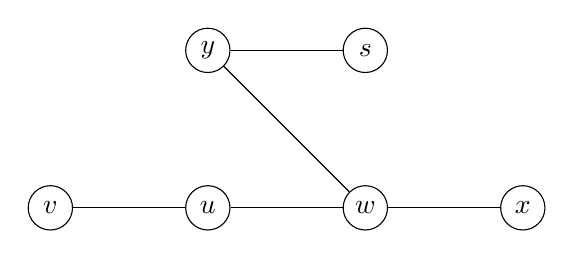
\begin{tikzpicture}[scale=2]
            \node (s) at (2,1) {$s$};
            \node (u) at (0,0) {$v$};
            \node (v) at (1,0) {$u$};
            \node (w) at (2,0) {$w$};
            \node (x) at (3,0) {$x$};
            \node (y) at (1,1) {$y$};
            \draw (u) -- (v);
            \draw (v) -- (w);
            \draw (w) -- (x);
            \draw (w) -- (y);
            \draw (y) -- (s);
        \end{tikzpicture}
    \end{center}
    Find a vertex cover $C$ of $T$ that includes the vertex $v$. 
    Now, explain why the set $C' = (C \setminus \{v\}) \cup \{u\}$ obtained from your $C$ by removing $v$ and adding (if it is not already present) $u$ is also a vertex cover of $T$.
    \item Now prove this property in general. That is, let $T$ be an arbitrary tree, suppose that $C$ is a vertex cover of $T$, and suppose that $C$ contains a leaf vertex $v$. 
    Let $u$ be the unique neighbor of $v$ in $T$, and let $C' = (C \setminus \{v\}) \cup \{u\}$ be the set of vertices obtained from $C$ by obtained from $C$ by removing $v$ and adding (if it is not already present) $u$. Carefully explain why $C'$ is a vertex cover of $T$.
\end{enumerate}

\begin{proof}[Answer]
    %%%%%%%%%%%%%%%%%%%%%%%%%%%%%%%%%%%%%%%%%%%%%%%%%%%%%%%%%%%%%%%%%%%%%%%%%%%%%%%
    % YOUR ANSWER GOES HERE: type your answer in below                             %
    %%%%%%%%%%%%%%%%%%%%%%%%%%%%%%%%%%%%%%%%%%%%%%%%%%%%%%%%%%%%%%%%%%%%%%%%%%%%%%%
\end{proof}


\end{required}

%%%%%%%%%%%%%%%%%%%%%%%%%%%%%%%%%%%%%%%%%%%%%%%%%%

\end{document} % NOTHING AFTER THIS LINE IS PART OF THE DOCUMENT